% Options for packages loaded elsewhere
\PassOptionsToPackage{unicode}{hyperref}
\PassOptionsToPackage{hyphens}{url}
%
\documentclass[
  ignorenonframetext,
  serif,
  professionalfont,
  usenames,
  dvipsnames,
  aspectratio = 169]{beamer}
\usepackage{pgfpages}
\setbeamertemplate{caption}[numbered]
\setbeamertemplate{caption label separator}{: }
\setbeamercolor{caption name}{fg=normal text.fg}
\beamertemplatenavigationsymbolsempty
% Prevent slide breaks in the middle of a paragraph
\widowpenalties 1 10000
\raggedbottom
\setbeamertemplate{part page}{
  \centering
  \begin{beamercolorbox}[sep=16pt,center]{part title}
    \usebeamerfont{part title}\insertpart\par
  \end{beamercolorbox}
}
\setbeamertemplate{section page}{
  \centering
  \begin{beamercolorbox}[sep=12pt,center]{part title}
    \usebeamerfont{section title}\insertsection\par
  \end{beamercolorbox}
}
\setbeamertemplate{subsection page}{
  \centering
  \begin{beamercolorbox}[sep=8pt,center]{part title}
    \usebeamerfont{subsection title}\insertsubsection\par
  \end{beamercolorbox}
}
\AtBeginPart{
  \frame{\partpage}
}
\AtBeginSection{
  \ifbibliography
  \else
    \frame{\sectionpage}
  \fi
}
\AtBeginSubsection{
  \frame{\subsectionpage}
}
\usepackage{amsmath,amssymb}
\usepackage{lmodern}
\usepackage{ifxetex,ifluatex}
\ifnum 0\ifxetex 1\fi\ifluatex 1\fi=0 % if pdftex
  \usepackage[T1]{fontenc}
  \usepackage[utf8]{inputenc}
  \usepackage{textcomp} % provide euro and other symbols
\else % if luatex or xetex
  \usepackage{unicode-math}
  \defaultfontfeatures{Scale=MatchLowercase}
  \defaultfontfeatures[\rmfamily]{Ligatures=TeX,Scale=1}
\fi
% Use upquote if available, for straight quotes in verbatim environments
\IfFileExists{upquote.sty}{\usepackage{upquote}}{}
\IfFileExists{microtype.sty}{% use microtype if available
  \usepackage[]{microtype}
  \UseMicrotypeSet[protrusion]{basicmath} % disable protrusion for tt fonts
}{}
\makeatletter
\@ifundefined{KOMAClassName}{% if non-KOMA class
  \IfFileExists{parskip.sty}{%
    \usepackage{parskip}
  }{% else
    \setlength{\parindent}{0pt}
    \setlength{\parskip}{6pt plus 2pt minus 1pt}}
}{% if KOMA class
  \KOMAoptions{parskip=half}}
\makeatother
\usepackage{xcolor}
\IfFileExists{xurl.sty}{\usepackage{xurl}}{} % add URL line breaks if available
\IfFileExists{bookmark.sty}{\usepackage{bookmark}}{\usepackage{hyperref}}
\hypersetup{
  pdftitle={Multivariate regression models for Twin data},
  pdfauthor={Prof.~Wagner Hugo Bonat},
  hidelinks,
  pdfcreator={LaTeX via pandoc}}
\urlstyle{same} % disable monospaced font for URLs
\newif\ifbibliography
\usepackage{color}
\usepackage{fancyvrb}
\newcommand{\VerbBar}{|}
\newcommand{\VERB}{\Verb[commandchars=\\\{\}]}
\DefineVerbatimEnvironment{Highlighting}{Verbatim}{commandchars=\\\{\}}
% Add ',fontsize=\small' for more characters per line
\newenvironment{Shaded}{}{}
\newcommand{\AlertTok}[1]{\textcolor[rgb]{1.00,0.00,0.00}{#1}}
\newcommand{\AnnotationTok}[1]{\textcolor[rgb]{0.00,0.50,0.00}{#1}}
\newcommand{\AttributeTok}[1]{#1}
\newcommand{\BaseNTok}[1]{#1}
\newcommand{\BuiltInTok}[1]{#1}
\newcommand{\CharTok}[1]{\textcolor[rgb]{0.00,0.50,0.50}{#1}}
\newcommand{\CommentTok}[1]{\textcolor[rgb]{0.00,0.50,0.00}{#1}}
\newcommand{\CommentVarTok}[1]{\textcolor[rgb]{0.00,0.50,0.00}{#1}}
\newcommand{\ConstantTok}[1]{#1}
\newcommand{\ControlFlowTok}[1]{\textcolor[rgb]{0.00,0.00,1.00}{#1}}
\newcommand{\DataTypeTok}[1]{#1}
\newcommand{\DecValTok}[1]{#1}
\newcommand{\DocumentationTok}[1]{\textcolor[rgb]{0.00,0.50,0.00}{#1}}
\newcommand{\ErrorTok}[1]{\textcolor[rgb]{1.00,0.00,0.00}{\textbf{#1}}}
\newcommand{\ExtensionTok}[1]{#1}
\newcommand{\FloatTok}[1]{#1}
\newcommand{\FunctionTok}[1]{#1}
\newcommand{\ImportTok}[1]{#1}
\newcommand{\InformationTok}[1]{\textcolor[rgb]{0.00,0.50,0.00}{#1}}
\newcommand{\KeywordTok}[1]{\textcolor[rgb]{0.00,0.00,1.00}{#1}}
\newcommand{\NormalTok}[1]{#1}
\newcommand{\OperatorTok}[1]{#1}
\newcommand{\OtherTok}[1]{\textcolor[rgb]{1.00,0.25,0.00}{#1}}
\newcommand{\PreprocessorTok}[1]{\textcolor[rgb]{1.00,0.25,0.00}{#1}}
\newcommand{\RegionMarkerTok}[1]{#1}
\newcommand{\SpecialCharTok}[1]{\textcolor[rgb]{0.00,0.50,0.50}{#1}}
\newcommand{\SpecialStringTok}[1]{\textcolor[rgb]{0.00,0.50,0.50}{#1}}
\newcommand{\StringTok}[1]{\textcolor[rgb]{0.00,0.50,0.50}{#1}}
\newcommand{\VariableTok}[1]{#1}
\newcommand{\VerbatimStringTok}[1]{\textcolor[rgb]{0.00,0.50,0.50}{#1}}
\newcommand{\WarningTok}[1]{\textcolor[rgb]{0.00,0.50,0.00}{\textbf{#1}}}
\usepackage{graphicx}
\makeatletter
\def\maxwidth{\ifdim\Gin@nat@width>\linewidth\linewidth\else\Gin@nat@width\fi}
\def\maxheight{\ifdim\Gin@nat@height>\textheight\textheight\else\Gin@nat@height\fi}
\makeatother
% Scale images if necessary, so that they will not overflow the page
% margins by default, and it is still possible to overwrite the defaults
% using explicit options in \includegraphics[width, height, ...]{}
\setkeys{Gin}{width=\maxwidth,height=\maxheight,keepaspectratio}
% Set default figure placement to htbp
\makeatletter
\def\fps@figure{htbp}
\makeatother
\setlength{\emergencystretch}{3em} % prevent overfull lines
\providecommand{\tightlist}{%
  \setlength{\itemsep}{0pt}\setlength{\parskip}{0pt}}
\setcounter{secnumdepth}{-\maxdimen} % remove section numbering
%-----------------------------------------------------------------------
% Logo na capa.

\titlegraphic{
  \vspace{-1em}
  % 
\includegraphics[height=1.2cm]{config/omega-logo.png}
  
\includegraphics[height=1.8cm]{config/logo-duas-cores.png}
  % 
\includegraphics[height=1.8cm]{config/logo-contorno.png}
  % 
\includegraphics[height=1.8cm]{config/linkedin-logo-da-pagina.png}
}

% \providecommand{\tightlist}{%
%   \setlength{\itemsep}{0pt}\setlength{\parskip}{0pt}}
% ATTENTION: Redefine o comando acima que é definido pelo template.
% \renewcommand{\tightlist}{}
\renewcommand{\tightlist}{%
  \setlength{\itemsep}{0\baselineskip}
  \setlength{\parskip}{0.25\baselineskip}
}
%-----------------------------------------------------------------------

% \usepackage{xltxtra}
%
% \setbeamerfont{title page}{family=\fontspec{Oswald}}
\setbeamerfont{title}{family=\fontspec{Oswald-Bold}}
\setbeamerfont{subtitle}{family=\fontspec{Oswald-Medium}}
\setbeamerfont{frametitle}{family=\fontspec{Oswald-Bold}}

% \setbeamerfont{title in head/foot}{family=\fontspec{Oswald-Medium}}
% \setbeamerfont{author in head/foot}{family=\fontspec{Oswald-Medium}}
\setbeamerfont{date in head/foot}{family=\fontspec{Oswald-Light}}
\setbeamerfont{section in head/foot}{family=\fontspec{Oswald-Light}}
\setbeamerfont{subsection in head/foot}{family=\fontspec{Oswald-Light}}

\setromanfont{Cardo}
\setsansfont{Cardo}
\setmonofont{inconsolata}

% Font for code. ----------------------------
% \usepackage[scaled=.75]{beramono}
% \usepackage{inconsolata}

% ATTENTION: needs complile with xelatex: `$ xelatex file.tex`
% \usepackage{fontspec}
% \setmonofont{M+ 1m}
% \setmonofont{M+ 1mn}
% \setmonofont{M+ 2m}

%-----------------------------------------------------------------------

% \usepackage{lmodern}
\usepackage{amssymb, amsmath}
\usepackage[makeroom]{cancel}
% \usepackage{ifxetex, ifluatex}
\usepackage{fixltx2e} % provides \textsubscript
%\usepackage[utf8]{inputenc}
\usepackage[shorthands=off, main=brazil]{babel}
\usepackage{graphicx}
\usepackage{xcolor}
\usepackage{setspace}
\usepackage{comment}
\usepackage{icomma}
\usepackage{multirow}

%-----------------------------------------------------------------------
% Algumas configurações.

\setlength{\parindent}{0pt}
\setlength{\parskip}{6pt plus 2pt minus 1pt}
\setlength{\emergencystretch}{3em}  % prevent overfull lines
% \providecommand{\tightlist}{%
%   \setlength{\itemsep}{0pt}\setlength{\parskip}{0pt}}
\setcounter{secnumdepth}{0}

% Espaço vertical para o ambiente `quote`.
\let\oldquote\quote
\let\oldendquote\endquote
\renewenvironment{quote}{%
  \vspace{1em}\oldquote}{%
  \oldendquote\vspace{1em}}

%-----------------------------------------------------------------------
% Espaçamento entre items para itemize, enumerate e description.

% % itemize.
% \let\itemopen\itemize
% \let\itemclose\enditemize
% \renewenvironment{itemize}{%
%   \itemopen\addtolength{\itemsep}{0.25\baselineskip}}{\itemclose}
%
% % enumerate.
% \let\enumopen\enumerate
% \let\enumclose\endenumerate
% \renewenvironment{enumerate}{%
%   \enumopen\addtolength{\itemsep}{0.25\baselineskip}}{\enumclose}
%
% % description.
% \let\descopen\description
% \let\descclose\enddescription
% \renewenvironment{description}{%
%   \descopen\addtolength{\itemsep}{0.25\baselineskip}}{\descclose}

%-----------------------------------------------------------------------

% \usepackage[hang]{caption}
\usepackage{caption}
\captionsetup{font=footnotesize,
  labelfont={color=mycolor1, footnotesize},
  labelsep=period}

% \providecommand{\tightlist}{%
%   \setlength{\itemsep}{0pt}\setlength{\parskip}{0pt}}

%-----------------------------------------------------------------------
% Imagem de fundo.

\usepackage{tikz}

% Caminho para a imagem de fundo com aspecto 16x9.
% \def\pathtobg{config/wallpapertip_gray-wallpaper_877207.jpg}
\def\pathtobg{config/light-gray-background.jpg}
\ifx\pathtobg\undefined
\else
  \usebackgroundtemplate{
    \tikz[overlay, remember picture]
    \node[opacity=0.5,
          at=(current page.south east),
          anchor=south east,
          inner sep=0pt] {
            \includegraphics[height=\paperheight, width=\paperwidth]{\pathtobg}};
  }
\fi

%-----------------------------------------------------------------------
% Logo.

% \logo{
%   
\includegraphics[width=0.6cm]{config/omega-logo.png}
% }

%-----------------------------------------------------------------------
% Definições de esquema de cores.

% Ômega.
% Preto #191824    Azul #102C54    Amarelo #FBCD1D    Magenta #EB0D6A
% http://www.color-hex.com/color-palette/2018
\definecolor{mycolor1}{HTML}{102C54} % Título.
\definecolor{mycolor3}{HTML}{102C54} % Estrutura.
\definecolor{mycolor4}{HTML}{102C54} % Links.
\definecolor{mycolor2}{HTML}{191824} % Texto.
\definecolor{mycolor5}{HTML}{CDCDCD} % Preenchimentos.

\hypersetup{
  colorlinks=true,
  linkcolor=mycolor4,
  urlcolor=mycolor1,
  citecolor=mycolor1
}

%-----------------------------------------------------------------------
% ATTENTION: http://www.cpt.univ-mrs.fr/~masson/latex/Beamer-appearance-cheat-sheet.pdf

\usetheme{Boadilla}
\usecolortheme{default}

% \setbeamersize{text margin left=7mm, text margin right=7mm}
% \setbeamertemplate{frametitle}[default][left, leftskip=3mm]
% \addtobeamertemplate{frametitle}{\vspace{0.5em}}{}

\setbeamertemplate{caption}[numbered]
\setbeamertemplate{section in toc}[sections numbered]
\setbeamertemplate{subsection in toc}[subsections numbered]
\setbeamertemplate{sections/subsections in toc}[ball]{}
\setbeamertemplate{sections in toc}[ball]
\setbeamercolor{section number projected}{bg=mycolor1, fg=white}
\setbeamertemplate{blocks}[rounded]
\setbeamertemplate{navigation symbols}{}
\setbeamertemplate{frametitle continuation}{\gdef\beamer@frametitle{}}
% \setbeamertemplate{frametitle}[default][center]
% \setbeamertemplate{footline}[frame number]

\setbeamertemplate{enumerate items}[default]
\setbeamertemplate{itemize items}{\scriptsize\raise1.25pt\hbox{\donotcoloroutermaths$\blacktriangleright$}}

% Blocos.
% \addtobeamertemplate{block begin}{\vskip -\bigskipamount}{}
% \addtobeamertemplate{block end}{}{\vskip -\bigskipamount}
\addtobeamertemplate{block begin}{\vspace{0.5em}}{}
\addtobeamertemplate{block end}{}{\vspace{0.5em}}

% Rodapé.
\setbeamercolor{title in head/foot}{parent=subsection in head/foot}
\setbeamercolor{author in head/foot}{bg=mycolor4, fg=white}
\setbeamercolor{date in head/foot}{parent=subsection in head/foot, fg=mycolor3}

% Cabeçalho.
\setbeamercolor{section in head/foot}{bg=mycolor2, fg=mycolor4}
\setbeamercolor{subsection in head/foot}{bg=mycolor2, fg=white}

\setbeamercolor{title}{fg=mycolor1}       % Título dos slides.
\setbeamercolor{titlelike}{fg=title}
\setbeamercolor{subtitle}{fg=mycolor2}    % Subtítulo.
\setbeamercolor{institute in head/foot}{parent=palette primary} % Instituição.
\setbeamercolor{frametitle}{fg=mycolor1}  % De quadro.
\setbeamercolor{structure}{fg=mycolor3}   % Listas e rodapé.
\setbeamercolor{item projected}{bg=mycolor2}
\setbeamercolor{block title}{bg=mycolor5, fg=mycolor2}
\setbeamercolor{normal text}{fg=mycolor2} % Texto.
\setbeamercolor{caption name}{fg=normal text.fg}
% \setbeamercolor{footlinecolor}{fg=mycolor2, bg=mycolor5}
% \setbeamercolor{section in head/foot}{fg=mycolor2, bg=mycolor5}
\setbeamercolor{author in head/foot}{fg=white, bg=mycolor1}
\setbeamercolor{section in foot}{fg=mycolor4, bg=mycolor5}
\setbeamercolor{date in foot}{fg=mycolor4, bg=mycolor5}
\setbeamercolor{block title}{fg=white, bg=mycolor1}
\setbeamercolor{block body}{fg=black, bg=white!80!gray}
\setbeamercolor{block body}{fg=black, bg=white!80!gray}

% To remove empty brackets of \institution.
\makeatletter
\setbeamertemplate{footline}{
  \leavevmode%
  \hbox{%
    \begin{beamercolorbox}[
      wd=0.3\paperwidth, ht=2.25ex, dp=1ex, right]{author in head/foot}%
      \usebeamerfont{author in head/foot}\insertshortauthor{}\hspace*{1ex}
    \end{beamercolorbox}%
    \begin{beamercolorbox}[
      wd=0.6\paperwidth, ht=2.25ex, dp=1ex, left]{section in foot}%
      \usebeamerfont{title in head/foot}\hspace*{1ex}\insertshorttitle{}
      % \usebeamerfont{title in head/foot}\hspace*{1ex}\insertframetitle{}
    \end{beamercolorbox}%
    \begin{beamercolorbox}[
      wd=0.1\paperwidth, ht=2.25ex, dp=1ex, right]{date in foot}%
      \insertframenumber{}\hspace*{2ex}
    \end{beamercolorbox}
  }%
  \vskip0pt%
}
\makeatother

%-----------------------------------------------------------------------

% \usepackage{hyphenat}
\usepackage{changepage}

% Slide para o título das seções.
\AtBeginSection[]{
  \begin{frame}
    % \vfill
    \vspace{4cm}
    % \centering
    % \begin{beamercolorbox}[sep = 8pt, center, shadow = true, rounded = true]{title}
    \begin{beamercolorbox}{title}
      \begin{columns}
        \column{0.7\linewidth}
        {\LARGE\textbf \insertsectionhead}
      \end{columns}
    \end{beamercolorbox}
    \vfill
  \end{frame}
}

%-----------------------------------------------------------------------
%---- preamble-chunk.tex -----------------------------------------------

% Knitr.

% ATTENTION: this needs `\usepackage{xcolor}'.
\definecolor{color_line}{HTML}{333333}
\definecolor{color_back}{HTML}{DDDDDD}
% \definecolor{color_back}{HTML}{FF0000}

% ATTENTION: usa o fancyvrb.
% https://ctan.math.illinois.edu/macros/latex/contrib/fancyvrb/doc/fancyvrb-doc.pdf
% R input.
\usepackage{tcolorbox}
\ifcsmacro{Highlighting}{
  % Statment if it exists. ------------------
  \DefineVerbatimEnvironment{Highlighting}{Verbatim}{
    % frame=lines,     % Linha superior e inferior.
    % framesep=1ex,    % Distância da linha para o texto.
    % framerule=0.5pt, % Espessura da linha.
    % rulecolor=\color{color_line},
    % numbers=right,
    fontsize=\footnotesize, % Tamanho da fonte.
    baselinestretch=0.9,   % Espaçamento entre linhas.
    commandchars=\\\{\}}
  % Margens do ambiente `Shaded'.
  % \fvset{listparameters={\setlength{\topsep}{-1em}}}
  % \renewenvironment{Shaded}{\vspace{-1ex}}{\vspace{-2ex}}
  \renewenvironment{Shaded}{
    \vspace{2pt}
    \begin{tcolorbox}[
      boxrule=0pt,      % Espessura do contorno.
      colframe=gray!10, % Cor do contorno.
      colback=gray!10,  % Cor de fundo da caixa.
      % arc=1em,          % Raio para contornos arredondados.
      sharp corners,
      % boxsep=0.5em,     % Margem interna.
      left=3pt, right=3pt, top=3pt, bottom=3pt, % Margens internas.
      % grow to left by=0mm,
      grow to right by=6pt,
      ]
    }{
    \end{tcolorbox}
    \vspace{-3pt}
    }
  }{
  % Statment if it not exists. --------------
}

% R output e todo `verbatim'.
\makeatletter
\def\verbatim@font{\linespread{0.9}\normalfont\ttfamily\footnotesize}
\makeatother

% Cor de fundo e margens do `verbatim'.
\let\oldv\verbatim
\let\oldendv\endverbatim

% \def\verbatim{%
%   \par\setbox0\vbox\bgroup % Abre grupo.
%   \vspace{-5px}            % Reduz margem superior.
%   \oldv                    % Chama abertura do verbatim.
% }
% \def\endverbatim{%
%   \oldendv                 % Chama encerramento do verbatim.
%   % \vspace{0cm}           % Controla margem inferior.
%   \egroup%\fboxsep5px      % Fecha grupo.
%   \noindent{\colorbox{color_back}{\usebox0}}\par
% }

%-----------------------------------------------------------------------
%---- preamble-commands.tex --------------------------------------------

% Para fazer texto em duas colunas.
\newcommand{\mytwocolumns}[4]{
  % #1: Line width fraction for the left column , e.g. 0.5.
  % #2: Line width fraction for the right column.
  % #3: Content for the left column.
  % #4: Content for the right column.
  \begin{columns}[c]
    \begin{column}{#1\linewidth} %----------- left.
      #3
    \end{column} %--------------------------- left.
    \begin{column}{#2\linewidth} %----------- right.
      #4
    \end{column} %--------------------------- right.
  \end{columns}
}

%-----------------------------------------------------------------------
% Para fazer duas colunas no Rmd.

% Center vertical align.
\def\beginAHalfColumn{\begin{minipage}{0.49\textwidth}}%
\def\beginAlmostHalfColumn{\begin{minipage}{0.45\textwidth}}%
\def\beginAQuarterColumn{\begin{minipage}{0.23\textwidth}}%
\def\beginThreeQuartersColumn{\begin{minipage}{0.72\textwidth}}%
\def\beginAThirdColumn{\begin{minipage}{0.31\textwidth}}%
\def\beginTwoThirdsColumn{\begin{minipage}{0.64\textwidth}}%
\def\endColumns{\end{minipage}}%

% Top vertical align.
\def\beginAHalfColumnT{\begin{minipage}[t]{0.49\textwidth}}%
\def\beginAlmostHalfColumnT{\begin{minipage}[t]{0.45\textwidth}}%
\def\beginAQuarterColumnT{\begin{minipage}[t]{0.23\textwidth}}%
\def\beginThreeQuartersColumnT{\begin{minipage}[t]{0.72\textwidth}}%
\def\beginAThirdColumnT{\begin{minipage}[t]{0.31\textwidth}}%
\def\beginTwoThirdsColumnT{\begin{minipage}[t]{0.64\textwidth}}%

%---------------------------------------------------------------------
% Ambientes para frases como e sem imagem.

\newcommand{\myquote}[3]{
  % #1: caminho para a imagem.
  % #2: a frase/quotation.
  % #3: o autor.
  \begin{center}
    \begin{minipage}[c]{0.19\linewidth}
      \begin{center}
        \includegraphics[height=2.5cm]{#1}
      \end{center}
    \end{minipage}
    \begin{minipage}[c]{0.7\linewidth}
      \begin{flushright}
        \textit{#2}
        \vspace{1ex}

        -- #3
      \end{flushright}
    \end{minipage}
  \end{center}
}

\newcommand{\myphrase}[2]{
  % #1: a frase/quotation.
  % #2: o autor.
  \begin{center}
    \begin{minipage}[c]{0.19\linewidth}
    \end{minipage}
    \begin{minipage}[c]{0.7\linewidth}
      \begin{flushright}
        \textit{#1}
        \vspace{1ex}

        -- #2
      \end{flushright}
    \end{minipage}
  \end{center}
}

%-----------------------------------------------------------------------
% Comandos para texto em destaque.

% \newcommand{\hi}[1]{%
%   \textcolor{ubuntu_orange}{#1}\xspace
% }

\usepackage{xspace}

% URLs com letra miuda.
\newcommand{\myurl}[1]{%
  {\tiny \url{#1}}\xspace
}

% Botões.
\newcommand{\btn}[1]{%
  \beamergotobutton{#1}\xspace
}

% Texto grande centralizado.
\newcommand{\centertitle}[1]{%
  \begin{center}
    {\LARGE \bfseries \hi{#1}}
  \end{center}
}

%-----------------------------------------------------------------------
\ifluatex
  \usepackage{selnolig}  % disable illegal ligatures
\fi

\title{Multivariate regression models for Twin data}
\subtitle{Analysis of Twin Data in Health Science · Session IV}
\author{Prof.~Wagner Hugo Bonat}
\date{}
\institute{Ômega Data Science \textbar{} Online School of Data Science}

\begin{document}
\frame{\titlepage}

\hypertarget{motivation}{%
\section{Motivation}\label{motivation}}

\begin{frame}{Heredity and variation}
\protect\hypertarget{heredity-and-variation}{}
\beginAHalfColumn

\begin{itemize}
\tightlist
\item
  Genetic epidemiology is impelled by three basic questions:

  \begin{enumerate}
  \tightlist
  \item
    Why isn't everyone the same?
  \item
    Why are children like their parents?
  \item
    Why aren't children from the same parents all alike?
  \end{enumerate}
\item
  \textbf{Main goal: Isolate/Separate sources of variation!}
\end{itemize}

\endColumns
\beginAHalfColumn

\begin{itemize}
\tightlist
\item
  Variation is everywhere!
\end{itemize}

\begin{figure}

{\centering 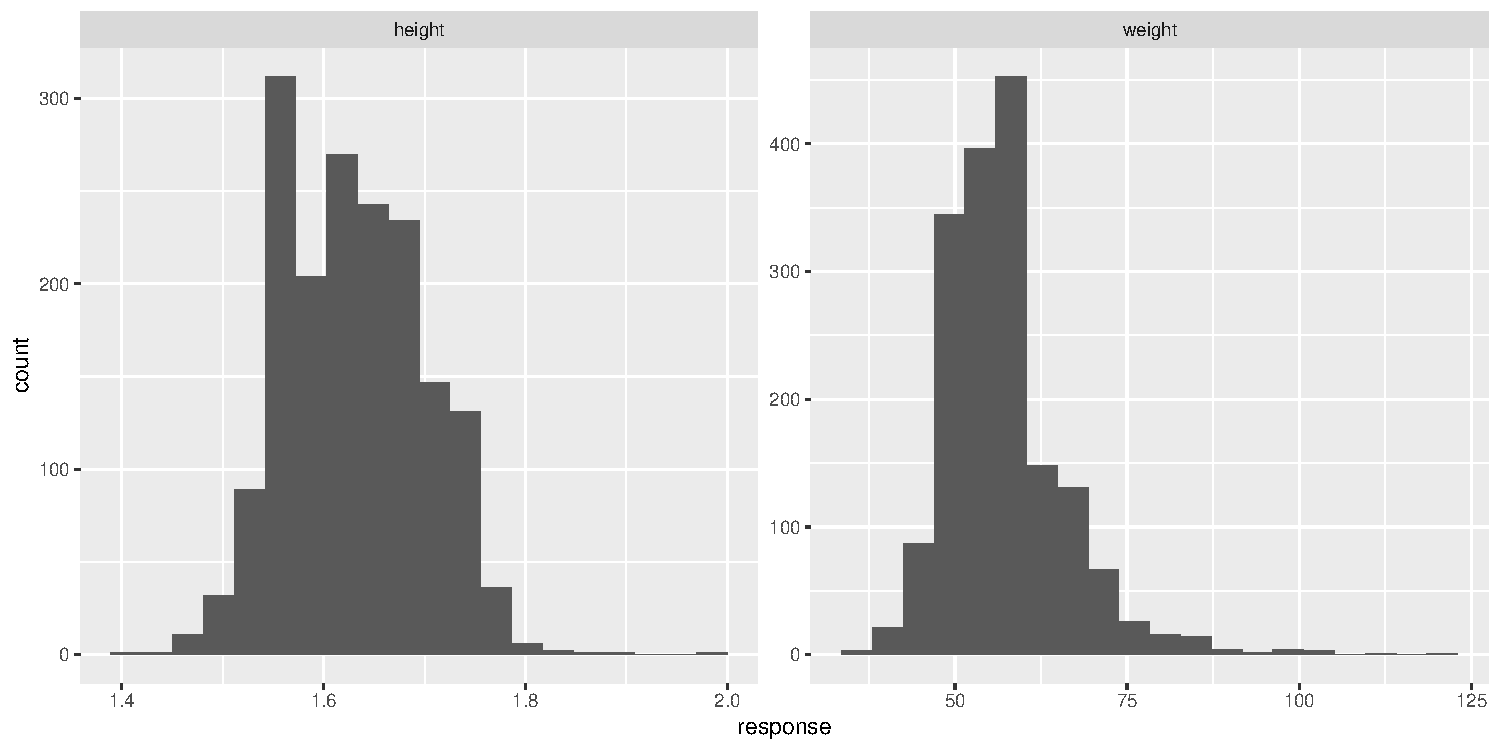
\includegraphics[width=1\linewidth]{Slides_files/figure-beamer/unnamed-chunk-2-1} 

}

\caption{Histogram of height and weight.}\label{fig:unnamed-chunk-2}
\end{figure}

\endColumns
\end{frame}

\begin{frame}[fragile]{Motivating dataset: Anthropometric measures}
\protect\hypertarget{motivating-dataset-anthropometric-measures}{}
\beginAHalfColumn

\begin{itemize}
\tightlist
\item
  Anthropometric measurements (weight and height).
\item
  861 twin pairs: 327 DZ (dizygotic) and 534 MZ (monozygotic).
\item
  Bivariate continuous traits.
\item
  Covariates: age and group.
\item
  Available as an example in the OpenMx package (Neale, et al., 2016).
\item
  Easy access from the \texttt{mglm4twin} package.
\end{itemize}

\endColumns
\beginAHalfColumn

\begin{figure}

{\centering 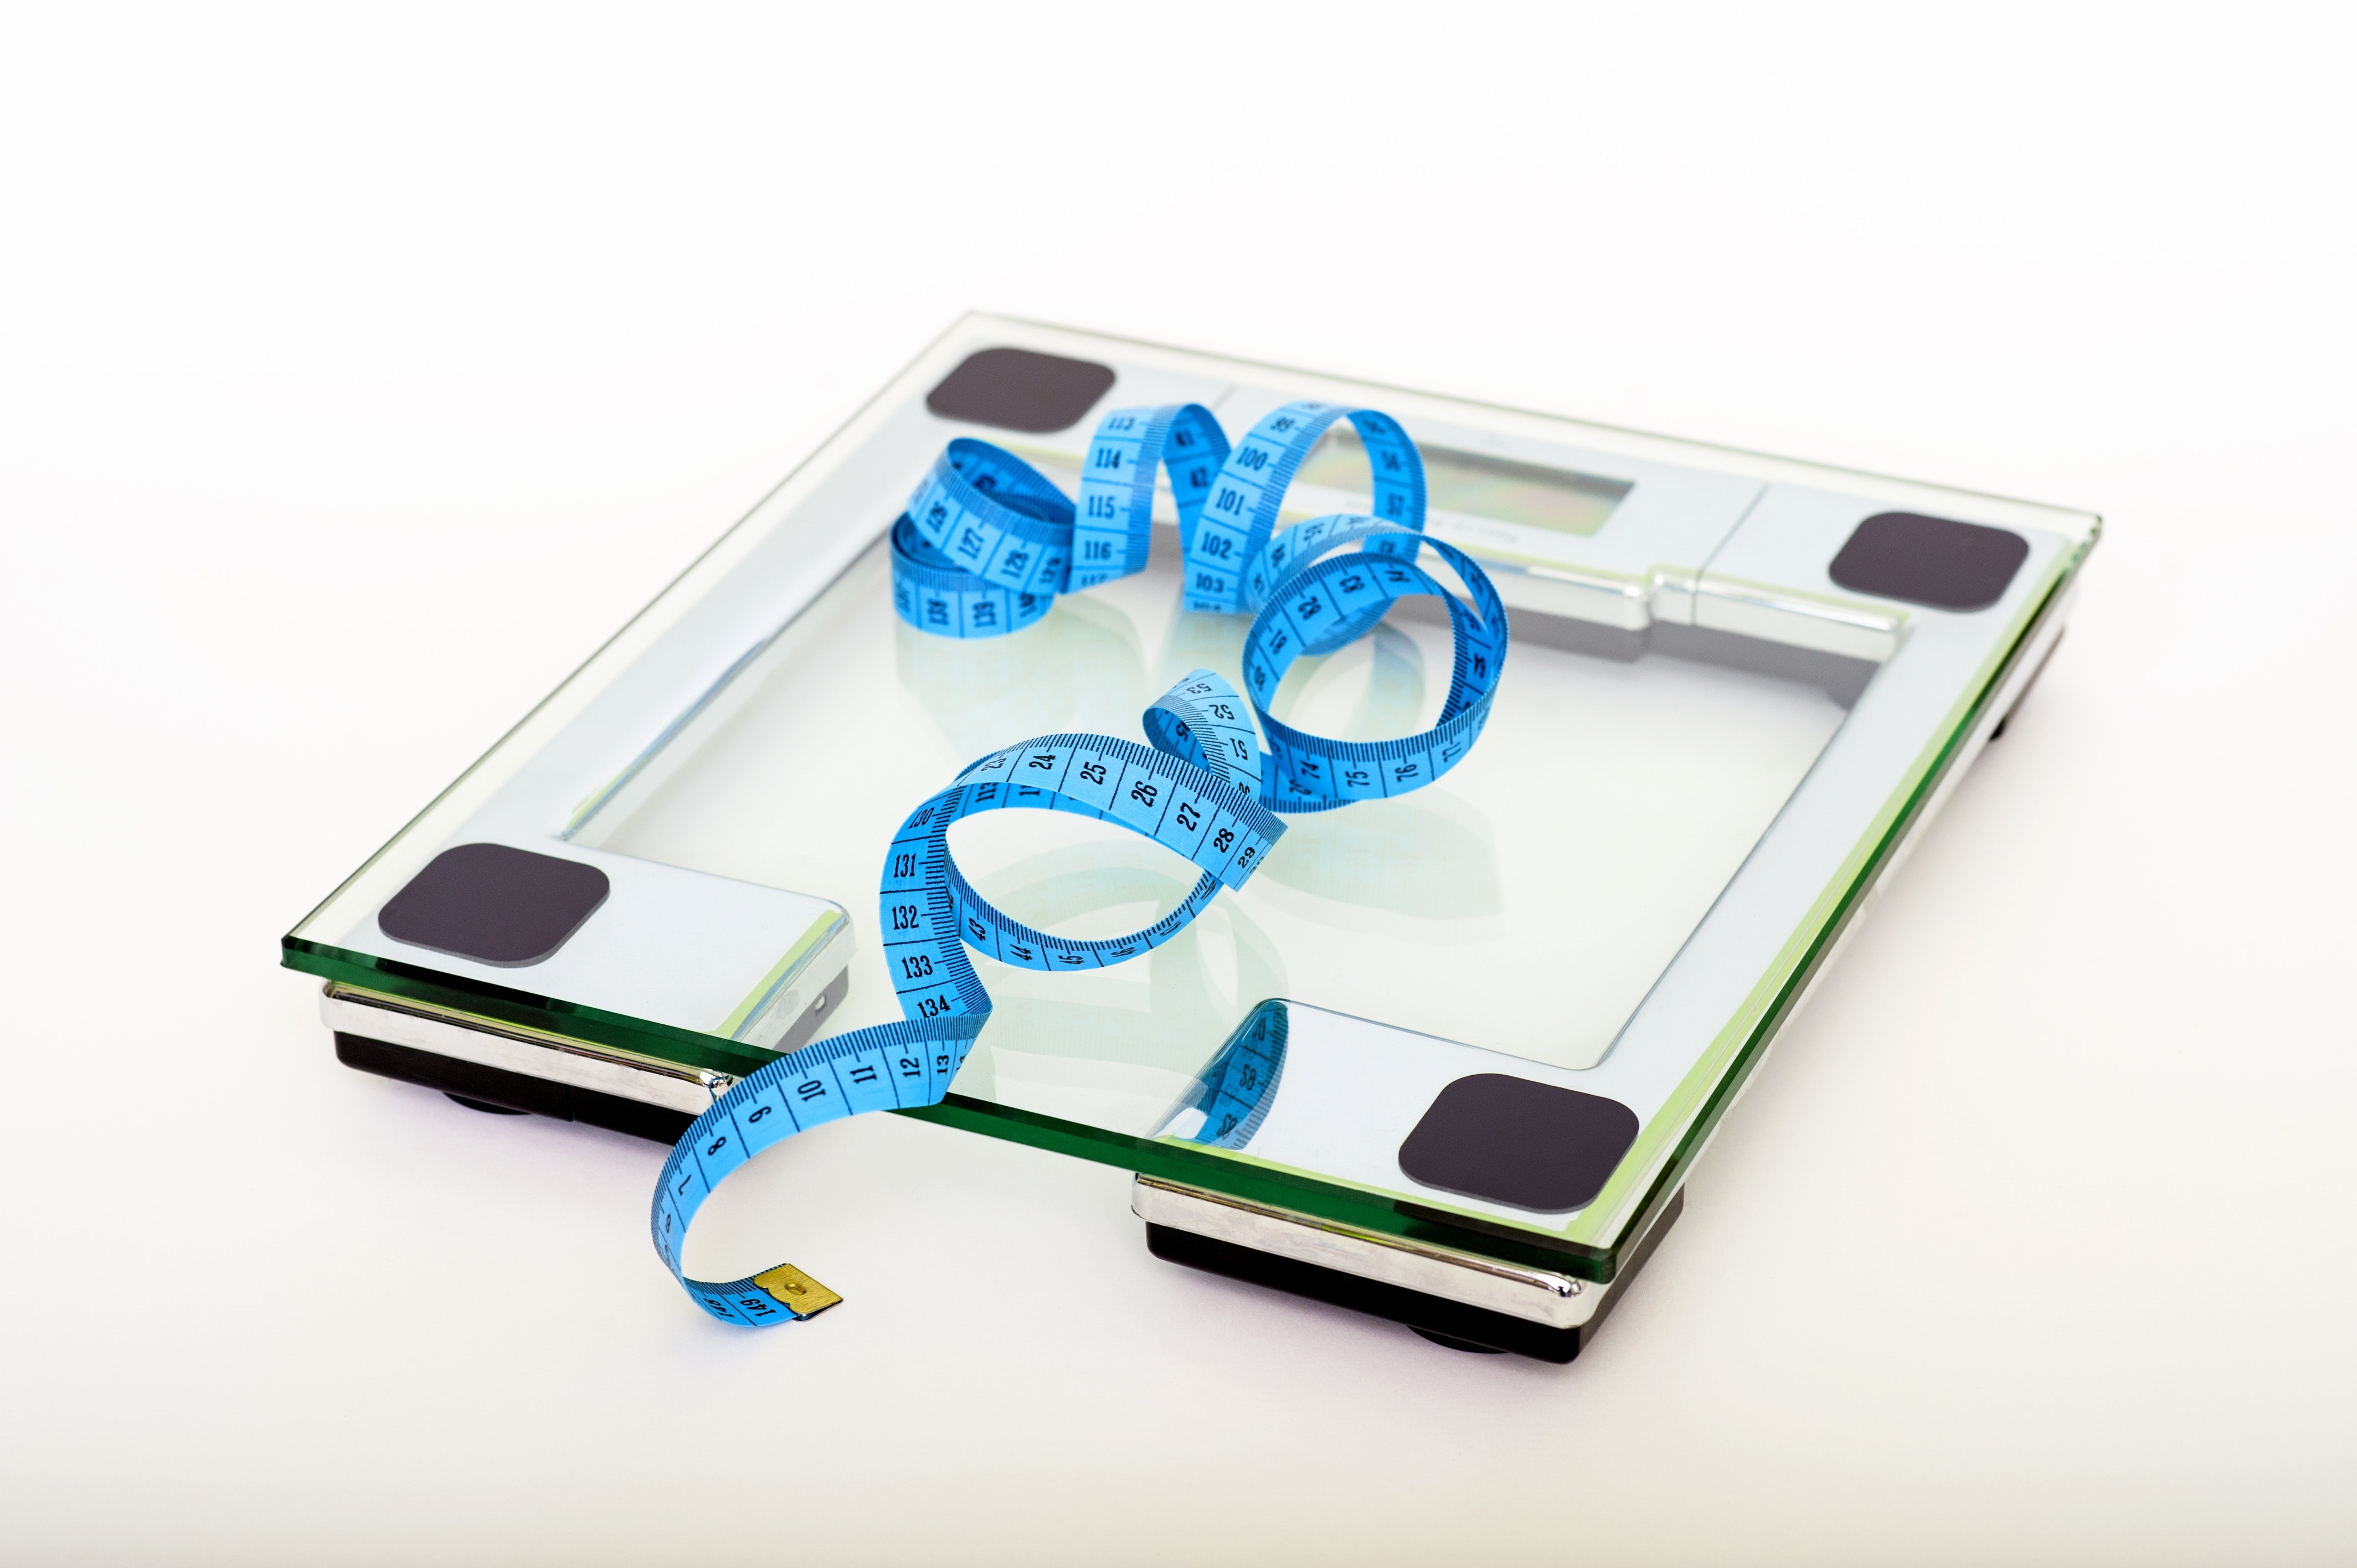
\includegraphics[width=0.8\linewidth]{./img/balanca} 

}

\caption{Photo by Pixabay.}\label{fig:unnamed-chunk-3}
\end{figure}

\endColumns
\end{frame}

\begin{frame}[fragile]{Motivating dataset: Anthropometric measures}
\protect\hypertarget{motivating-dataset-anthropometric-measures-1}{}
\begin{itemize}
\tightlist
\item
  The dataset
\end{itemize}

\begin{Shaded}
\begin{Highlighting}[]
\FunctionTok{library}\NormalTok{(mglm4twin)}
\FunctionTok{data}\NormalTok{(anthro)}
\FunctionTok{glimpse}\NormalTok{(anthro)}
\end{Highlighting}
\end{Shaded}

\begin{verbatim}
## Rows: 1,722
## Columns: 6
## $ weight    <int> 62, 55, 66, 73, 51, 44, 52, 57, 54, 54, 58, 57, ~
## $ height    <dbl> 1.6499, 1.6299, 1.6599, 1.7000, 1.7300, 1.5698, ~
## $ age       <int> 24, 24, 20, 20, 20, 20, 26, 26, 20, 20, 22, 22, ~
## $ Group     <fct> DZ, DZ, DZ, DZ, DZ, DZ, DZ, DZ, DZ, DZ, DZ, DZ, ~
## $ Twin      <int> 535, 535, 536, 536, 537, 537, 538, 538, 539, 539~
## $ Twin_pair <int> 1, 2, 1, 2, 1, 2, 1, 2, 1, 2, 1, 2, 1, 2, 1, 2, ~
\end{verbatim}
\end{frame}

\begin{frame}{Graphing and Quantifying Familial Resemblance}
\protect\hypertarget{graphing-and-quantifying-familial-resemblance}{}
\begin{figure}

{\centering 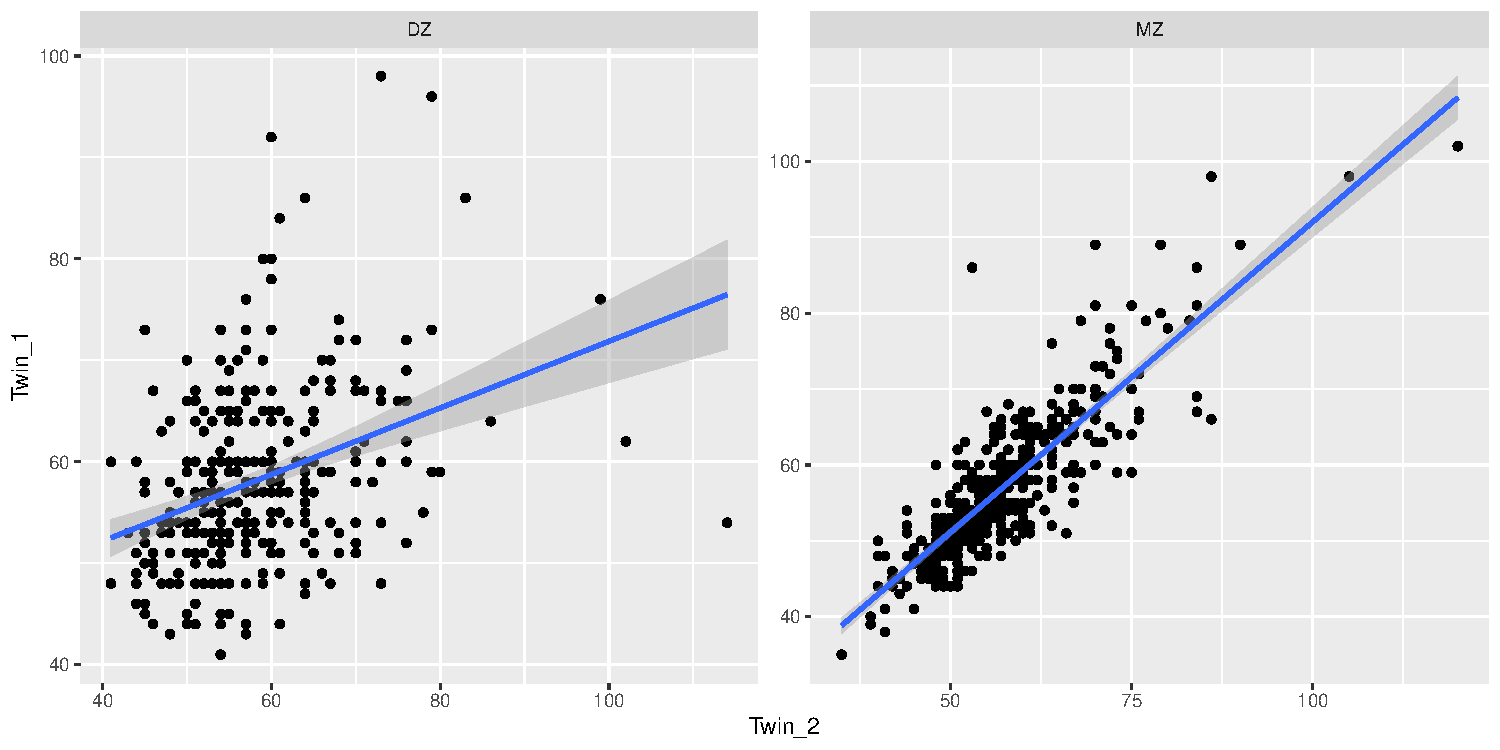
\includegraphics[width=0.8\linewidth]{Slides_files/figure-beamer/unnamed-chunk-5-1} 

}

\caption{Dispersion diagram by zygosity · Trait weight.}\label{fig:unnamed-chunk-5}
\end{figure}
\end{frame}

\begin{frame}{Multiple traits}
\protect\hypertarget{multiple-traits}{}
\begin{figure}

{\centering 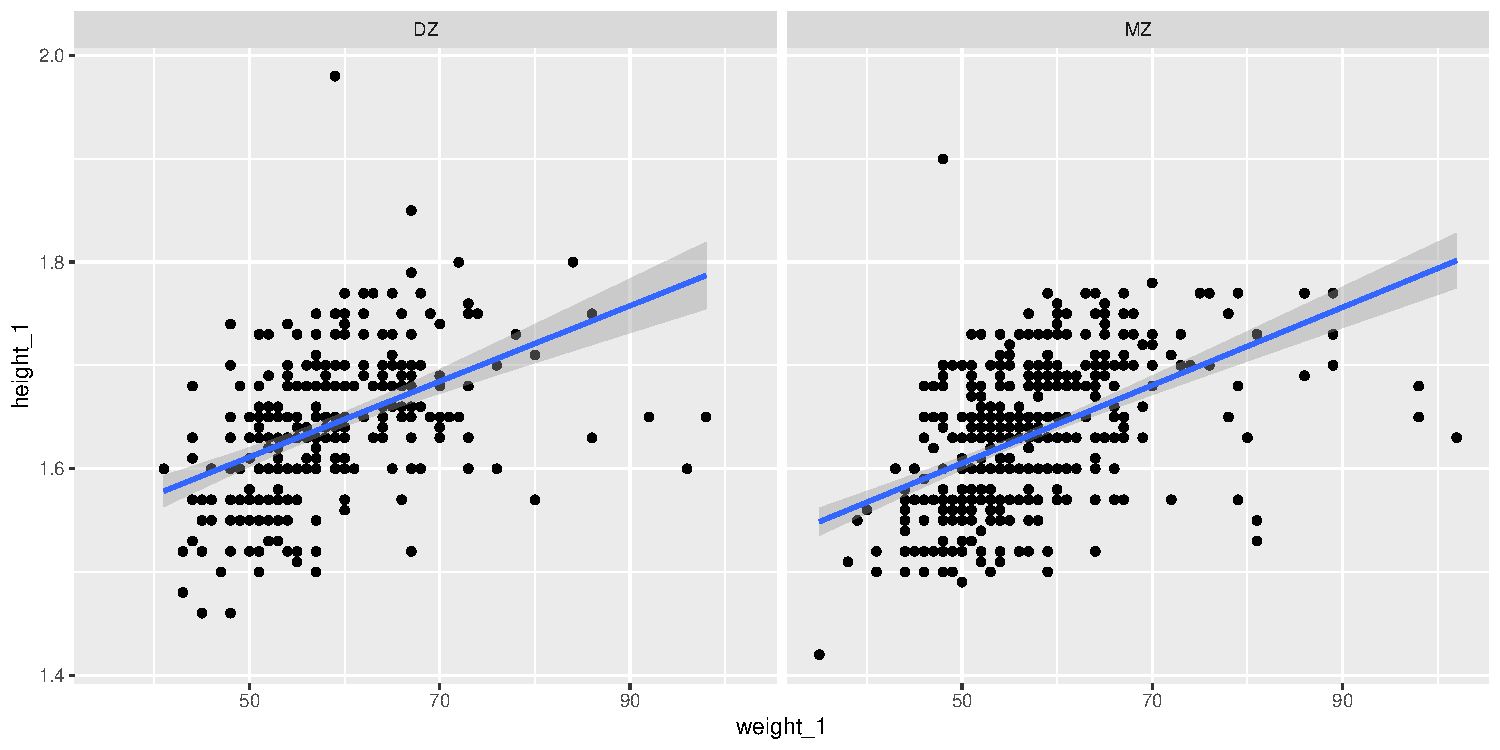
\includegraphics[width=0.8\linewidth]{Slides_files/figure-beamer/unnamed-chunk-6-1} 

}

\caption{Dispersion diagram by zygosity · Weight vs Height.}\label{fig:unnamed-chunk-6}
\end{figure}
\end{frame}

\begin{frame}{Building and Fitting Models}
\protect\hypertarget{building-and-fitting-models}{}
\begin{figure}

{\centering 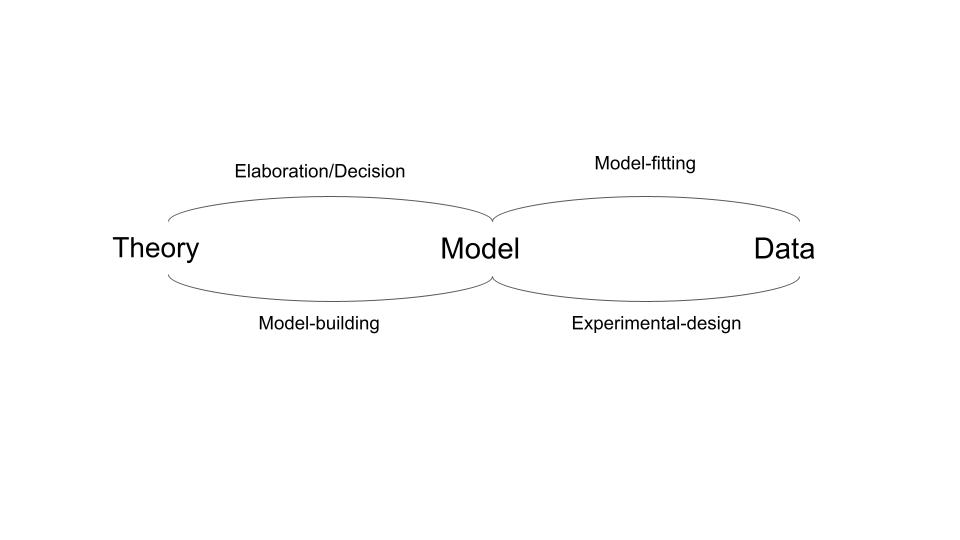
\includegraphics[width=0.75\linewidth]{./img/model} 

}

\caption{Diagram of the interrelationship between theory, model and empirical observation. Adapted from Neale and Maes (1992).}\label{fig:unnamed-chunk-7}
\end{figure}
\end{frame}

\begin{frame}{Challenges for model-building in Twin data analyses}
\protect\hypertarget{challenges-for-model-building-in-twin-data-analyses}{}
\beginAHalfColumn

\begin{itemize}
\tightlist
\item
  Decompose sources of variation

  \begin{enumerate}
  \tightlist
  \item
    Genetic Effects.
  \item
    Environmental Effects.
  \item
    Genotype-Environment Interaction.
  \end{enumerate}
\item
  Traits types

  \begin{enumerate}
  \tightlist
  \item
    Binary and binomial data.
  \item
    Bounded data and continuous proportions.
  \item
    Under-, equi- and over-dispersed count data.
  \item
    Semi-continuous data (continuous \(+\) mass at zero).
  \item
    Symmetric and assymetric continuous data.
  \end{enumerate}
\item
  Multiple traits of mixed types.
\end{itemize}

\endColumns
\beginAHalfColumn

\begin{figure}

{\centering 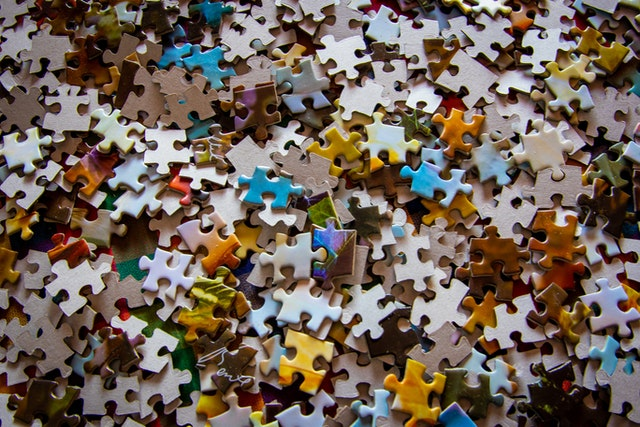
\includegraphics[width=0.8\linewidth]{./img/blocks} 

}

\caption{Photo by Magda Ehlers from Pexels.}\label{fig:unnamed-chunk-8}
\end{figure}

\endColumns
\end{frame}

\begin{frame}{Importance and statistical approaches}
\protect\hypertarget{importance-and-statistical-approaches}{}
\begin{itemize}
\tightlist
\item
  Multivariate twin and family studies are important tools to:

  \begin{enumerate}
  \tightlist
  \item
    Determine traits inheritance;
  \item
    Determine the influence of genetic and environmental effects on
    traits.
  \end{enumerate}
\item
  Statistical challenge:

  \begin{enumerate}
  \tightlist
  \item
    Model the covariance structure to take into account the genetic and
    environmental structures induced by the twin and family designs.
  \end{enumerate}
\item
  Orthodox approaches:

  \begin{enumerate}
  \tightlist
  \item
    Structural equation modelling (SEM); 2. Linear mixed models (LMM).
  \end{enumerate}
\item
  Main limitations of SEM and LMM:

  \begin{enumerate}
  \tightlist
  \item
    Both deal only with Gaussian (symmetric) data;
  \item
    Standard computational implementations are difficult to adapt for
    the analysis of twin and family data.
  \end{enumerate}
\end{itemize}
\end{frame}

\hypertarget{multivariate-generalized-linear-models}{%
\section{Multivariate generalized linear
models}\label{multivariate-generalized-linear-models}}

\begin{frame}[fragile]{Multivariate generalized linear models (mglm):
What is it?}
\protect\hypertarget{multivariate-generalized-linear-models-mglm-what-is-it}{}
\begin{itemize}
\tightlist
\item
  Flexible statistical modelling framework to deal with multivariate
  traits.
\item
  Tailored for twin and family data by Bonat and Hjelmborg (2022).
\item
  The mglm approach deals with:

  \begin{enumerate}
  \tightlist
  \item
    Binary and binomial data;
  \item
    Bounded data and continuous proportions;
  \item
    Under-, equi- and over-dispersed count data.
  \item
    Semi-continuous data (continuous \(+\) mass at zero);
  \item
    Symmetric and assymetric continuous data.
  \item
    Combination of all the previous mentioned data.
  \end{enumerate}
\item
  Estimation and inference based on estimating functions (Bonat and
  Jorgense, 2016).
\item
  Computational implementation available through the \texttt{mglm4twin}
  package.
\end{itemize}
\end{frame}

\begin{frame}{Multivariate generalized linear models (mglm):
Non-standard features}
\protect\hypertarget{multivariate-generalized-linear-models-mglm-non-standard-features}{}
\beginAHalfColumn

\begin{itemize}
\tightlist
\item
  Extend standard measures of genetic studies such as:

  \begin{enumerate}
  \tightlist
  \item
    Bivariate heritability, environmentability and common
    environmentability;
  \item
    Genetic, environmental and phenotypic correlations,
  \end{enumerate}
\end{itemize}

to non-Gaussian traits.

\begin{itemize}
\tightlist
\item
  Provide a flexible framework for modelling the dispersion parameters
  as functions of potential covariates.
\item
  Provide software implementation in \texttt{R}.
\end{itemize}

\endColumns
\beginAHalfColumn

\begin{figure}

{\centering 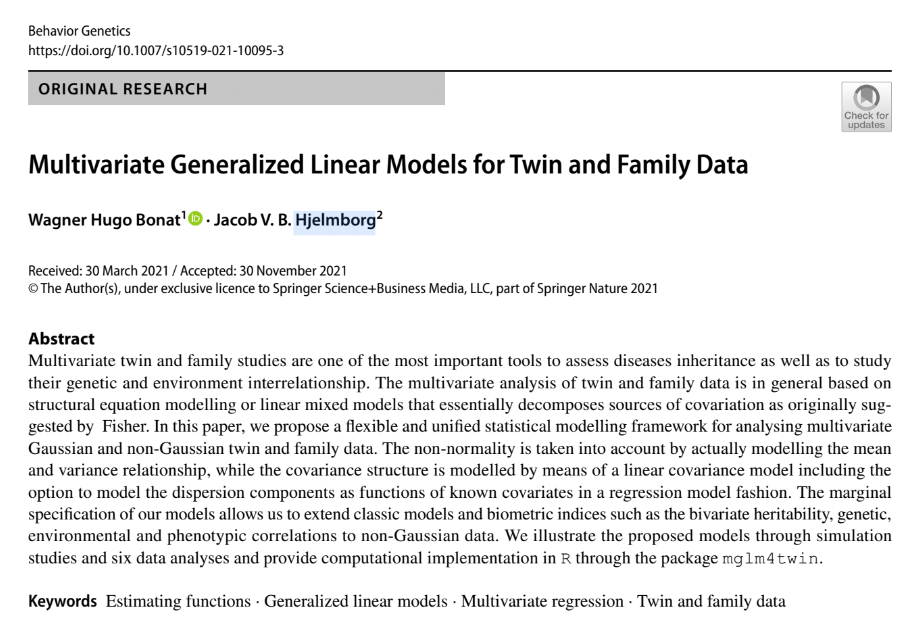
\includegraphics[width=0.8\linewidth]{./img/Paper} 

}

\end{figure}

\endColumns
\end{frame}

\hypertarget{multivariate-generalized-linear-models-for-twin-data}{%
\section{Multivariate generalized linear models for twin
data}\label{multivariate-generalized-linear-models-for-twin-data}}

\begin{frame}{Generalized linear models for twin data}
\protect\hypertarget{generalized-linear-models-for-twin-data}{}
\begin{itemize}
\tightlist
\item
  Let \(Y_{i}\) be a \(2 \times 1\) random vector of the i\(th\) twin
  pair for \(i = 1, \ldots, n\).
\item
  Let \(\mathbf{x}_{i} = (x_{i1}, \ldots, x_{ik})^{\top}\) denote a
  \(2 \times k\) design matrix.
\item
  Let \(\boldsymbol{\beta}\) be a \(k \times 1\) parameter vector.
\item
  Consider \((y_{i},\mathbf{x}_{i})\), where \(y_{i}'s\) are iid
  realizations of \(Y_{i}\) according to an \textbf{unspecified}
  bivariate distribution, whose expectation and variance are given by
  \begin{eqnarray}
  \label{modelGLM}
  \mathrm{E}(Y_i) &=& \mu_i = g^{-1}(\mathbf{x}_{i}^{\top}\beta)  \nonumber \\
  \mathrm{var}(Y_i) &=& \Sigma_i = \mathrm{V}(\mu_i;p)^{\frac{1}{2}}\Omega\mathrm{V}(\mu_i;p)^{\frac{1}{2}}.
  \end{eqnarray}
\item
  \(g\) some suitable link function.
\item
  \(\mathrm{V}(\mu_i;p) = \mathrm{diag}(\vartheta(\mu_i;p))\), where
  \(\vartheta(\mu_i;p)\) describes the mean and variance relation and
  \(p\) is the power parameter (to be estimated).
\item
  \(\Omega\) is a \(2 \times 2\) dispersion matrix.
\end{itemize}
\end{frame}

\begin{frame}{Generalized linear models for twin data}
\protect\hypertarget{generalized-linear-models-for-twin-data-1}{}
\begin{itemize}
\tightlist
\item
  The models decompose the covariance matrix into two components.
  \[ \mathrm{var}(Y_i) = \Sigma_i = \mathrm{V}(\mu_i;p)^{\frac{1}{2}}\Omega\mathrm{V}(\mu_i;p)^{\frac{1}{2}}\]
\item
  \(\mathrm{V}(\mu_i;p)\) deals with non-Gaussianity.
\item
  Variance/dispersion functions

  \begin{enumerate}
  \tightlist
  \item
    \(\vartheta(\mu;p) = \mu^p\) characterizes the Tweedie distribution
    deals with continuous and semi-continuous data. Gaussian \((p=0)\),
    Gamma \((p=2)\) and inverse Gaussian \((p=3)\).
  \item
    \(\vartheta(\mu;p) = \mu + \tau \mu^p\) characterizes the
    Poisson-Tweedie distribution deals with count data. Neyman-type A
    \((p=1)\), negative binomial \((p=2)\) and PIG \((p=3)\).
  \item
    \(\vartheta(\mu;p) = \mu^p (1- \mu)^p\) generalization of binomial
    variance function deals with binary, binomial and bounded data.
  \end{enumerate}
\item
  \(p\) is an index that identifies the distribution.
\item
  In practice, we estimate \(p\) which works as an automatic model
  selection.
\end{itemize}
\end{frame}

\begin{frame}{Generalized linear models for twin data}
\protect\hypertarget{generalized-linear-models-for-twin-data-2}{}
\begin{itemize}
\tightlist
\item
  \(\Omega\) models the dependence between twin pair.
\item
  Polygenic ACDE model has the components \begin{equation*}
  \label{components}
  \mathrm{A} = \begin{bmatrix}
  1 & a\\ 
  a & 1
  \end{bmatrix}, \quad
  \mathrm{C} = \begin{bmatrix}
  1 & 1\\ 
  1 & 1
  \end{bmatrix}, \quad
  \mathrm{D} = \begin{bmatrix}
  1 & d\\ 
  d & 1
  \end{bmatrix}\quad \text{and} \quad
  \mathrm{E} \begin{bmatrix}
  1 & 0\\ 
  0 & 1
  \end{bmatrix}.
  \end{equation*}
\item
  Dispersion matrix is modelled by \begin{equation}
  \label{linearCovariance}
  \Omega = \tau_A \mathrm{A} + \tau_C \mathrm{C} + \tau_D \mathrm{D} + \tau_E \mathrm{E},
  \end{equation} where \(a=1\) and \(d = 1\) for MZ twins and
  \(a=\frac{1}{2}\) and \(d = \frac{1}{4}\) for DZ twins.
\item
  Plugging Eq.(\ref{linearCovariance}) in Eq.(\ref{modelGLM}), we have a
  flexible class of models to deal with twin data.
\item
  But, still only one trait.
\end{itemize}
\end{frame}

\begin{frame}{Multivariate GLMs for twin data}
\protect\hypertarget{multivariate-glms-for-twin-data}{}
\begin{itemize}
\tightlist
\item
  Let \(\mathbf{Y}_{ir}\) be the \(2 \times 1\) response vector of the
  r\(th\) trait for \(r = 1, \ldots, R\).
\item
  Let \(\mathbf{x}_{ir} = (x_{ir1}, \ldots, x_{irk})^{\top}\) be the
  \(2 \times k_r\) design matrix.
\item
  Let \(\boldsymbol{\beta}_r\) be the \(k_r \times 1\) parameter
  vectors.
\item
  Let \(\mathbf{Y}_i = (Y_{i1}^{\top}, \ldots, Y_{iR}^{\top}){^\top}\)
  denote the \(2R \times 1\) stacked vector of response variables.
\item
  Multivariate GLMs for twin data \begin{eqnarray}
  \label{modelMGLM}
  \mathrm{E}(\mathbf{Y}_i) &=& \boldsymbol{\mu}_{i} = (g_1^{-1}(\mathbf{x}_{i1}^{\top} \boldsymbol{\beta}_1), \ldots, g_{R}^{-1}(\mathbf{x}_{iR}^{\top} \boldsymbol{\beta}_R))  \nonumber \\
  \mathrm{var}(\mathbf{Y}_i) &=& \boldsymbol{\Sigma}_i = \mathrm{V}(\boldsymbol{\mu}_i;\boldsymbol{p})^{\frac{1}{2}}\boldsymbol{\Omega}\mathrm{V}(\boldsymbol{\mu}_i;\boldsymbol{p})^{\frac{1}{2}}.
  \end{eqnarray}
\item
  \(\mathrm{V}(\boldsymbol{\mu}_i; \boldsymbol{p}) = \mathrm{diag}(\vartheta_1(\mu_1;p_1), \ldots, \vartheta_R(\mu_R;p_R))\),
\item
  \(\boldsymbol{p} = (p_1, \ldots, p_R)\) is an \(R \times 1\) vector of
  power parameters.
\item
  \(\boldsymbol{\Omega}\) is a \(2R \times 2R\) dispersion matrix.
\end{itemize}
\end{frame}

\begin{frame}{Multivariate GLMs for twin data}
\protect\hypertarget{multivariate-glms-for-twin-data-1}{}
\begin{itemize}
\tightlist
\item
  Specification of \(\boldsymbol{\Omega}\) is crucial.
\item
  Let \(\boldsymbol{\nabla}_{r r^{\prime}}\) denote an \(R \times R\)
  matrix, whose entries \(r = r^{\prime}\) and \(r^{\prime} = r\) are
  equal to \(1\) and \(0\) elsewhere, for \(r = 1, \ldots, R\) and
  \(r^{\prime} \leq r\). \begin{eqnarray}
  \label{multACDE}
  \boldsymbol{\Omega} &=& 
  \tau_{A_{rr\prime}} \left\{ \boldsymbol{\nabla}_{rr\prime} \otimes \mathrm{A} \right\} +  
  \tau_{C_{rr\prime}} \left\{ \boldsymbol{\nabla}_{rr\prime} \otimes \mathrm{C} \right\} \nonumber \\ &+& 
  \tau_{D_{rr\prime}} \left\{ \boldsymbol{\nabla}_{rr\prime} \otimes \mathrm{D} \right\} +  
  \tau_{E_{rr\prime}} \left\{ \boldsymbol{\nabla}_{rr\prime} \otimes \mathrm{E} \right\},
  \end{eqnarray} where
  \(\tau_{A_{rr\prime}}, \tau_{C_{rr\prime}}, \tau_{D_{rr\prime}}\) and
  \(\tau_{E_{rr\prime}}\) are dispersion parameters associated with the
  additive genetic, common environment, dominance genetic and unique
  environment effects.
\end{itemize}
\end{frame}

\begin{frame}{Dispersion matrix}
\protect\hypertarget{dispersion-matrix}{}
\begin{itemize}
\item
  Bivariate case \begin{eqnarray*}
  \boldsymbol{\Omega} = &\tau_{A_{11}} & \nonumber
  \begin{bmatrix}
  \mathrm{A} & \mathrm{0} \\ 
  \mathrm{0} & \mathrm{0}
  \end{bmatrix} + \tau_{A_{22}}
  \begin{bmatrix}
  \mathrm{0} & \mathrm{0} \\ 
  \mathrm{0} & \mathrm{A}
  \end{bmatrix} + \tau_{A_{12}}
  \begin{bmatrix}
  \mathrm{0} & \mathrm{A} \\ 
  \mathrm{A} & \mathrm{0}
  \end{bmatrix} + \\ \nonumber
  & \tau_{C_{11}} &
  \begin{bmatrix}
  \mathrm{C} & \mathrm{0} \\ 
  \mathrm{0} & \mathrm{0}
  \end{bmatrix} + \tau_{C_{22}}
  \begin{bmatrix}
  \mathrm{0} & \mathrm{0} \\ 
  \mathrm{0} & \mathrm{C}
  \end{bmatrix} + \tau_{C_{12}}
  \begin{bmatrix}
  \mathrm{0} & \mathrm{C} \\ 
  \mathrm{C} & \mathrm{0}
  \end{bmatrix} + \\
  &\tau_{E_{11}}& 
  \begin{bmatrix}
  \mathrm{E} & \mathrm{0} \\ 
  \mathrm{0} & \mathrm{0}
  \end{bmatrix} + \tau_{E_{22}}
  \begin{bmatrix}
  \mathrm{0} & \mathrm{0} \\ 
  \mathrm{0} & \mathrm{E}
  \end{bmatrix} + \tau_{E_{12}}
  \begin{bmatrix}
  \mathrm{0} & \mathrm{E} \\ 
  \mathrm{E} & \mathrm{0}
  \end{bmatrix}.
  \end{eqnarray*}
\item
  Note: ACDE model is unidentifiable.
\end{itemize}
\end{frame}

\begin{frame}{Measures of interest}
\protect\hypertarget{measures-of-interest}{}
\begin{itemize}
\tightlist
\item
  Broad sense bivariate heritability, common environmentality and
  environmentality: \begin{eqnarray*}
  h_{rr^{\prime}} &=& \frac{\tau_{A_{rr^{\prime}}} + \tau_{D_{rr^{\prime}}} } {\tau_{A_{rr^{\prime}}} + \tau_{C_{rr^{\prime}}} + \tau_{E_{rr^{\prime}}} }, \\
  c_{rr^{\prime}} &=& \frac{\tau_{C_{rr^{\prime}}} } {\tau_{A_{rr^{\prime}}} + \tau_{C_{rr^{\prime}}} + \tau_{E_{rr^{\prime}}} } \quad \text{and} \quad \\
  e_{rr^{\prime}} &=& \frac{\tau_{E_{rr^{\prime}}} } {\tau_{A_{rr^{\prime}}} + \tau_{C_{rr^{\prime}}} + \tau_{E_{rr^{\prime}}} }.
  \end{eqnarray*}
\end{itemize}
\end{frame}

\begin{frame}{Measures of interest}
\protect\hypertarget{measures-of-interest-1}{}
\begin{itemize}
\item
  Genetic, common environmental and environmental correlations:
  \begin{eqnarray*}
  r_{G_{rr^{\prime}}} &=& \frac{ \tau_{A_{rr^{\prime}}} + \tau_{D_{rr^{\prime}}} }{ \sqrt{\tau_{A_{rr}} + \tau_{D_{rr}}} \sqrt{\tau_{A_{r^{\prime}r^{\prime}}} + \tau_{D_{r^{\prime}r^{\prime}}} } },  \\
  r_{C_{rr^{\prime}}} &=& \frac{ \tau_{C_{rr^{\prime}}} }{ \sqrt{\tau_{C_{rr}}} \sqrt{\tau_{C_{r^{\prime}r^{\prime}}} } } \quad \text{and} \quad
  r_{E_{rr^{\prime}}} = \frac{ \tau_{E_{rr^{\prime}}} }{ \sqrt{\tau_{E_{rr}}} \sqrt{\tau_{E_{r^{\prime}r^{\prime}}} } }.
  \end{eqnarray*}
\item
  Phenotypic correlation \begin{equation*}
  r_{P_{rr^{\prime}}} = \frac{\tau_{Prr^{\prime}}}{\sqrt{ \tau_{Prr}}\sqrt{ \tau_{Pr^{\prime}r^{\prime}}} },
  \end{equation*} where
  \(\tau_{Prr^{\prime}} = \tau_{Arr^{\prime}} + \tau_{C{rr^{\prime}}} + \tau_{D{rr^{\prime}}} + \tau_{E{rr^{\prime}}}.\)
\end{itemize}
\end{frame}

\begin{frame}{Modelling the dispersion parameters}
\protect\hypertarget{modelling-the-dispersion-parameters}{}
\begin{itemize}
\tightlist
\item
  Interest to model the component \(\tau_A\) in a regression model
  fashion.
\item
  Let \(\boldsymbol{z}_i\) be a \((2 \times q)\) design matrix.
  \begin{equation*}
  \boldsymbol{z}_i = \begin{bmatrix}
  1 & z_{i11} & \ldots & z_{i1q} \\ 
  1 & z_{i21} & \ldots & z_{i2q}
  \end{bmatrix}.
  \end{equation*}
\item
  Let
  \(\boldsymbol{\tau_A} = (\tau_A(0), \tau_A(1), \ldots, \tau_A(q))\)
  denote the \((q \times 1)\) vector of dispersion parameters.
\item
  Dispersion components associated to the additive genetic effect
  \begin{equation}
  \label{regdisp}
  \tau_{A(0)}
  \begin{bmatrix}
  1\\ 
  1
  \end{bmatrix} \circ \mathrm{A} + 
  \tau_{A(1)} 
  \begin{bmatrix}
  z_{i11}\\ 
  z_{i21}
  \end{bmatrix} \circ \mathrm{A} + \ldots 
  \tau_{A(q)} 
  \begin{bmatrix}
  z_{i1q}\\ 
  z_{i2q}
  \end{bmatrix} \circ \mathrm{A},
  \end{equation} where \(\circ\) denotes the Hadamard product.
\item
  All dispersion parameters can be modelled as in Eq.(\ref{regdisp}) and
  the model remains a linear covariance model.
\end{itemize}
\end{frame}

\hypertarget{estimation-and-inference}{%
\section{Estimation and Inference}\label{estimation-and-inference}}

\begin{frame}{Estimation and Inference}
\protect\hypertarget{estimation-and-inference-1}{}
\begin{itemize}
\tightlist
\item
  Estimation and inference is carried out using an estimating function
  approach.
\item
  Fitting procedure adapted from Bonat and J\o rgensen, 2016.
\item
  Quasi-score estimating functions for regression parameters.
\item
  Pearson estimating functions for power and dispersion parameters.
\item
  Computational implementation in \texttt{R} through the
  \texttt{mglm4twin}.
\item
  Available on github \texttt{https://github.com/wbonat/mglm4twin}.
\end{itemize}
\end{frame}

\hypertarget{data-analyses}{%
\section{Data analyses}\label{data-analyses}}

\begin{frame}{Data set 1: Bivariate dichotomous data}
\protect\hypertarget{data-set-1-bivariate-dichotomous-data}{}
\begin{itemize}
\tightlist
\item
  Bronchopulmonary dysplasia (BPD) and respiratory distress syndrome
  (RDS) on preterm infants.
\item
  Both diseases are lung related and expected to have a genetic
  component.
\item
  Dataset consists of \(200\) twin-pairs being \(137\) DZ and \(63\) MZ.
\item
  Covariates: birth weight (BW), gestation age (GA) and gender (1: male
  and 0: female).
\item
  Bivariate ACE model and its special cases as well as their univariate
  counterparts.
\end{itemize}
\end{frame}

\begin{frame}{Data set 1: Results}
\protect\hypertarget{data-set-1-results}{}
\begin{itemize}
\tightlist
\item
  Multivariate AE model provides the best balance between
  goodness-of-fit and complexity. \tiny

  \begin{table}[]
  \caption{Pseudo log-likelihood (\texttt{pll}) values along with the pseudo \textit{Akaike} (\texttt{pAIC}), Bayesian ($pBIC$) information criterion and degrees of freedom (df) by fitted models - Bivariate binary twin data.}
  \label{tab:dataset3}
  \begin{tabular}{lrrrrrrrr}
  \hline
  \multicolumn{1}{|l|}{\multirow{3}{*}{Criterion}} & \multicolumn{8}{c|}{Models}                                                                                                                                                                                   \\ \cline{2-9} 
  \multicolumn{1}{|l|}{}                           & \multicolumn{4}{c|}{Univariate}                                                                       & \multicolumn{4}{c|}{Multivariate}                                                                     \\ \cline{2-9} 
  \multicolumn{1}{|l|}{}                           & \multicolumn{1}{l|}{ACE} & \multicolumn{1}{l|}{CE} & \multicolumn{1}{l|}{AE} & \multicolumn{1}{l|}{E} & \multicolumn{1}{l|}{ACE} & \multicolumn{1}{l|}{CE} & \multicolumn{1}{l|}{AE} & \multicolumn{1}{l|}{E} \\ \hline
  pll  & $-323.03$ & $-334.97$ & $-324.22$ & $-359.99$ & $-311.86$ & $-323.82$ & $-312.90$ & $-347.59$ \\
  pAIC & $686.06$  & $705.94$  & $684.44$  & $751.98$  & $669.72$  & $687.64$  & $665.80$  & $729.18$   \\
  pBIC & $779.75$  & $742.04$  & $748.56$  & $774.86$  & $777.47$  & $781.33$  & $759.49$  & $808.82$ \\
  df   & $20$      & $18$      & $18$      & $16$      & $23$      & $20$      & $20$      &  $17$ \\ \hline            
  \end{tabular}
  \end{table}
\end{itemize}
\end{frame}

\begin{frame}{Data set 1: Results}
\protect\hypertarget{data-set-1-results-1}{}
\begin{table}[]
\caption{Parameter estimates and standard errors for some genetic and environment indices of interest - Bivariate binary twin data.}
\label{tab:dataset3gen}
\begin{tabular}{lrrr}
\hline
\multicolumn{1}{|l|}{\multirow{2}{*}{Indices}} & \multicolumn{3}{c|}{Traits} \\ \cline{2-4} 
\multicolumn{1}{|l|}{} & \multicolumn{1}{l|}{BPD} & \multicolumn{1}{l|}{RDS} & \multicolumn{1}{l|}{BPD $\times$ RDS} \\ \hline
Heritability            & $0.70(0.15)$ & $0.43(0.07)$ & $0.98(0.18)$ \\
Environmentality        & $0.30(0.15)$ & $0.57(0.07)$ & $0.02(0.18)$  \\
Genetic correlation     & $--$         & $--$         & $0.45(0.11)$ \\
Environment correlation & $--$         & $--$         & $0.01(0.11)$ \\ \hline                                        
\end{tabular}
\end{table}
\end{frame}

\begin{frame}{Data set 2: Bivariate continuous data}
\protect\hypertarget{data-set-2-bivariate-continuous-data}{}
\begin{itemize}
\tightlist
\item
  Traits of interest: body weight and height measures.
\item
  Data set consists of \(861\)\textasciitilde(\(327\) DZ and \(534\) MZ)
  twin-pairs.
\item
  These traits are well-known to be highly genetic determined and
  correlated.
\item
  Covariate age was used for modelling both the mean and covariance
  structures.
\item
  Responses and covariates were standardized (mean zero and variance
  one).
\end{itemize}
\end{frame}

\begin{frame}{Data set 2: Results}
\protect\hypertarget{data-set-2-results}{}
\begin{center}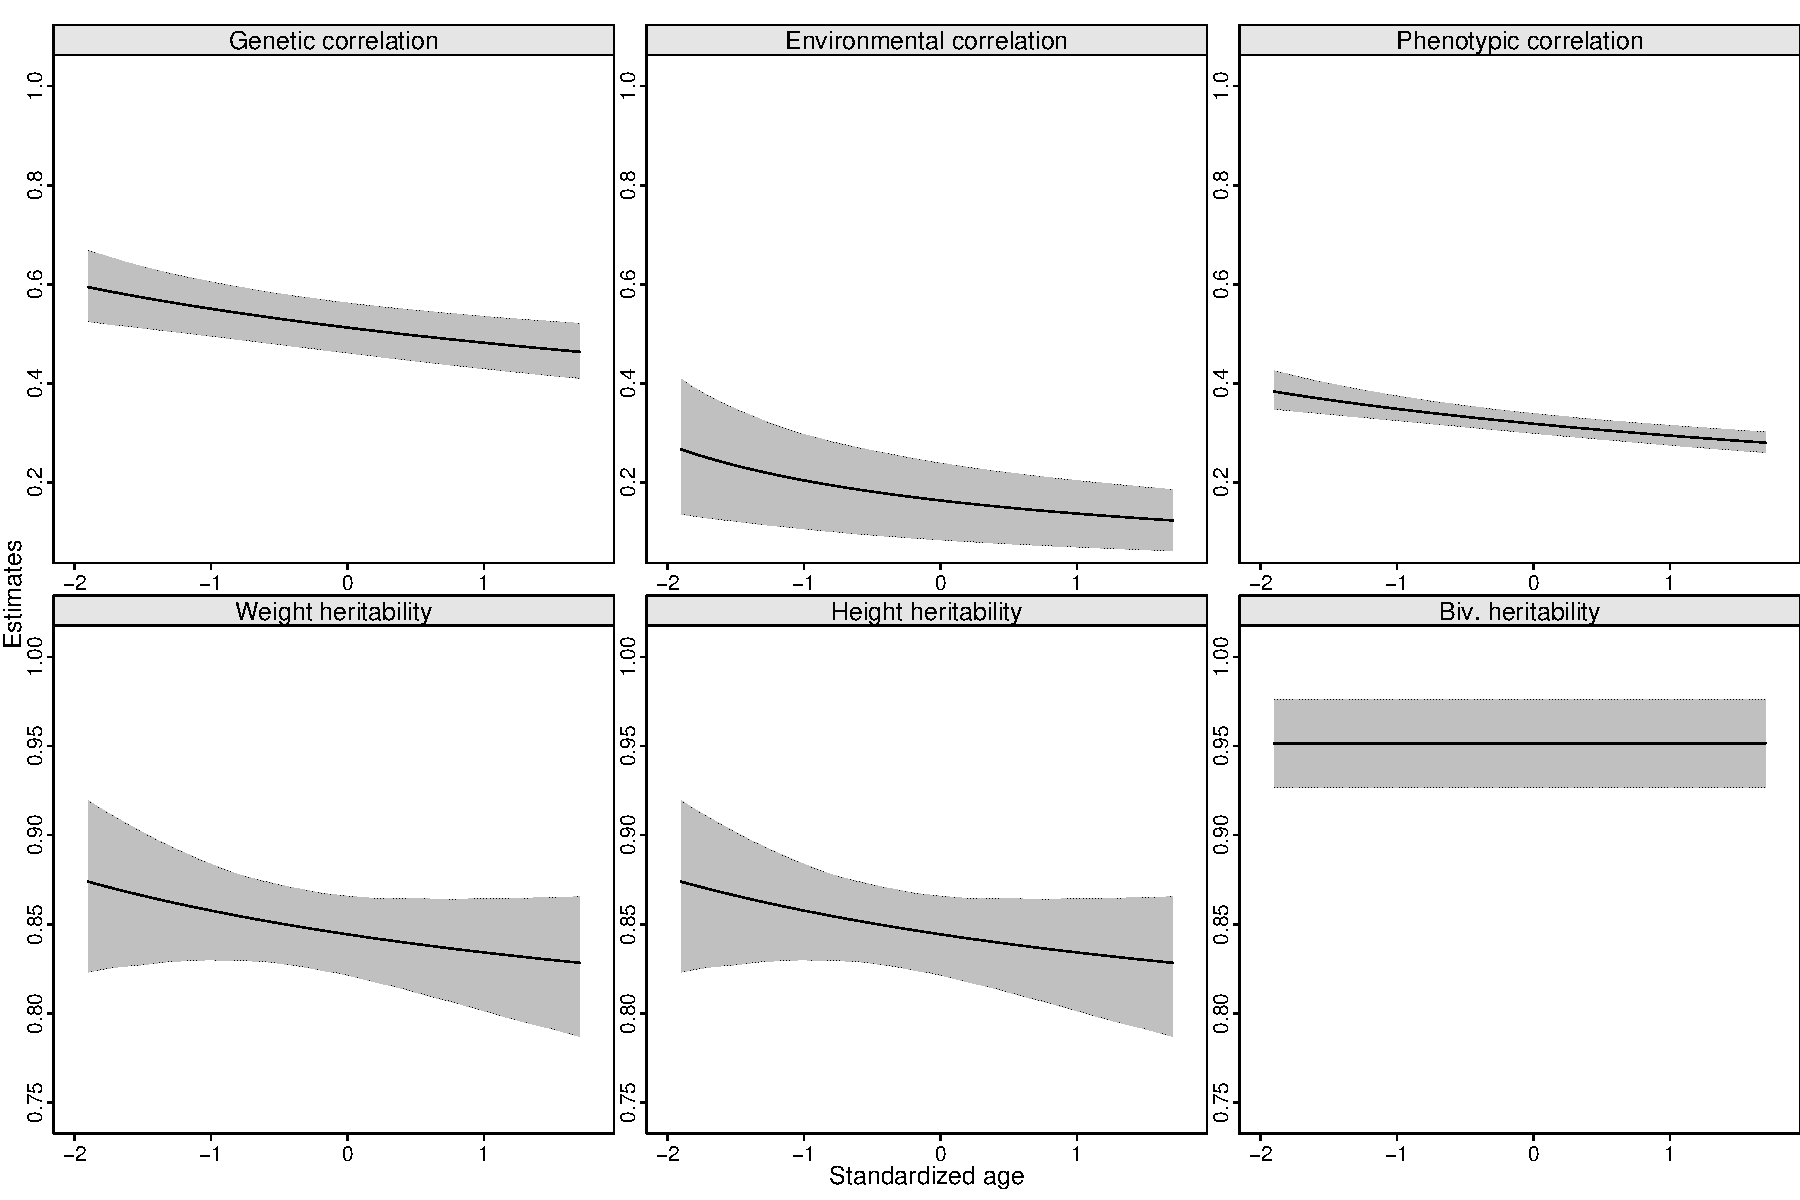
\includegraphics[width=0.65\linewidth]{img/FigDataset4} \end{center}
\end{frame}

\hypertarget{discussion}{%
\section{Discussion}\label{discussion}}

\begin{frame}{Main results}
\protect\hypertarget{main-results}{}
\begin{itemize}
\tightlist
\item
  Flexible multivariate statistical modelling framework to deal with
  twin data.
\item
  Second-moment assumptions.
\item
  General framework for estimation based on estimating function.
\item
  Efficient algorithms for estimation.
\item
  Asymptotic theory (Godambe Information).
\item
  General software implementation in \texttt{R} (\texttt{mglm4twin}
  package).
\item
  Extension of the main genetic measures to non-Gaussian data.
\item
  Future research topics

  \begin{enumerate}
  \tightlist
  \item
    Weighted estimating functions.
  \item
    Time to event data.
  \end{enumerate}
\item
  Check the webpage for more examples
  \href{http://www.leg.ufpr.br/~wagner/mglm4twin}{mglm4twin}.
\end{itemize}
\end{frame}

\end{document}
